\section{Introduction} Is it possible to characterize ``good'' representations
without specifying a task a priori? If so, does there exist a set of generic
priors which lead to these representations? In recent years state-of-the-art
results from supervised learning suggest that the most powerful representations
for solving specific tasks can be learned from the data itself. It has been
hypothesized that large collections of unprocessed and unlabeled data can be
used to learn generically useful representations. However the principles which
would lead to these representations in the realm of unsupervised learning
remain elusive. Temporal coherence is a form of weak supervision, which we
exploit to learn generic signal representations that are stable with respect to
the variability in natural video, including local deformations. 

Our main assumption is that data samples that are temporal neighbors are also
likely to be neighbors in the latent space. For example, adjacent frames in a
video sequence are more likely to be semantically similar than non-adjacent
frames. This assumption naturally leads to the slowness prior on features which
was introduced in SFA (\cite{SFA}). 

This prior has been successfully applied to metric learning, as a regularizer
in supervised learning, and in unsupervised learning
(\cite{DrLIM,DrLIMVideo,SFA}). A popular assumption in unsupervised learning is
that high dimensional data lies on a low dimensional manifold  parametrized by
the latent variables as in \cite{Bengio2012,CAE,DAE,SATAE}. In this case,
temporal sequences can be thought of as one-dimensional trajectories on this
manifold. Thus, an ensemble of sequences that pass through a common data sample
have the potential to reveal the local latent variable structure within a
neighborhood of that sample. 

Non-linear operators consisting of a redundant linear transformation followed
by a point-wise nonlinearity and a local pooling, are fundamental building
blocks in deep convolutional networks. This is due to their capacity to
generate local invariance while preserving discriminative information
(\cite{LeCun1998, JoanScat}). We justify that pooling operators are a natural
choice for our unsupervised learning architecture since they induce invariance
to local deformations. The resulting pooling auto-encoder model captures the
main source of variability in natural video sequences, which can be further
exploited by enforcing a convolutional structure. Experiments on YouTube data
show that one can learn pooling representations with good discrimination and
stability to observed temporal variability. We show that these features
represent a metric which we evaluate on retrieval and classification tasks. 

\section{Contributions and Prior Work} The problem of learning temporally
stable representations has been extensively studied in the literature, most
prominently in Slow Feature Analysis (SFA) and Slow Subspace Analysis (SSA)
(\cite{SFA,SSA,hyvarinen2003bubbles}). Works that learn slow features
distinguish themselves mainly in three ways: (1) how the features are
parametrized, (2) how the trivial (constant) solution is avoided, and (3)
whether or not additional priors such as independence or sparsity are imposed
on the learned features. 

The features presented in SFA take the form of a nonlinear transformation of
the input, specifically a quadratic expansion followed by a linear combination
using learned weights optimized for slowness (\cite{SFA}).  This
parametrization is equivalent to projecting onto a learned basis followed by
$L_2$ pooling. The recent work by \cite{complexCells} uses features which are
composed of projection onto a learned unitary basis followed by a local $L_2$
pooling in groups of two. 

Slow feature learning methods also differ in the way that they avoid the
trivial solution of learning to extract constant features. Constant features
are perfectly slow (invariant), however they are not informative
(discriminative) with respect to the input. All slow feature learning methods
must make a trade-off between the discriminability and stability of the learned
features in order to avoid trivial solutions. Slow Feature Analysis introduces
two additional constraints, namely that the learned features must have unit
variance and must be decorrelated from one another. In the work by
\cite{complexCells}, the linear part of the transformation into feature space
is constrained to be unitary. Enforcing that the transform be unitary implies
that it is invertible \emph{for all inputs}, and not just the data samples.
This unnecessarily limits the invariance properties of the transform and
precludes the possibility of learning over-complete bases. Since the pooling
operation following this linear transform has no trainable parameters,
including this constraint is sufficient to avoid the trivial solution. Metric
learning approaches (\cite{DrLIM}) can be used to perform dimensionality
reduction by optimizing a criteria which minimizes the distance between
temporally adjacent samples in the transformed space, while repelling
non-adjacent samples with a hinge loss, as explained in Section
\ref{sec:slowmetric}. The margin based contrastive term in DrLIM is explicitly
designed to only avoid the constant solution and provides no guarantee on how
informative the learned features are. Furthermore since distances grow
exponentially due to the curse of dimensionality, metric based contrastive
terms can be trivially satisfied in high dimensions.

Our approach uses a reconstruction criterion as a contrastive term. This
approach is most similar to the one taken by \cite{groupSparsity} when
optimizing group sparsity. In this work group-sparsity is replaced by slowness,
and multiple layers of convolutional slow features are trained. 

Several other studies combine the slowness prior with independence inducing
priors \cite{complexCells, Cadieu, zou2012deep}. For a detailed discussion on
the connection between independence and sparsity see \cite{Huyvarinen}.
However, our model maximizes the sparsity of the representation \emph{before}
the pooling operator. Our model can be interpreted as a sparse auto-encoder
additionally regularized by slowness through a local pooling operator.   

In this work we introduce the use of convolutional pooling architectures for
slow feature learning.  At small spatial scales, local translations comprise
the dominant source of variability in natural video; this is why many previous
works on slowness learn mainly locally translation-invariant features
(\cite{SFA,SSA,complexCells}). However, convolutional pooling architectures are
locally translation-invariant by design, which allows our model to learn
features that capture a richer class of invariances, beyond translation.
Finally, we demonstrate that nontrivial convolutional dictionaries can be
learned in the unsupervised setting using only stochastic gradient descent (on
mini-batches), despite their huge redundancy --- that is, without resorting to
alternating descent methods or iterative sparse inference algorithms. 


\section{Slowness as Metric Learning } \label{sec:slowmetric}

\begin{figure}
\centering
%\subfigure[ ]{
\begin{subfigure}[b]{0.49 \textwidth}
\centering
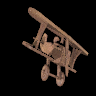
\includegraphics[scale=0.5]{./figures/slow/toyplane.png} 
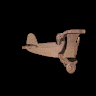
\includegraphics[scale=0.5]{./figures/slow/toyplane2.png} 
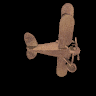
\includegraphics[scale=0.5]{./figures/slow/toyplane3.png}
        \caption{}
\label{fig:toyplane}
\end{subfigure}
%\caption{ }
%\end{figure} 
%
%\begin{figure}
%\centering 
%\begin{subfigure}[]
%\subfigure[ ]{
%\hspace{0.5cm}
\begin{subfigure}[b]{0.49 \textwidth}
\centering
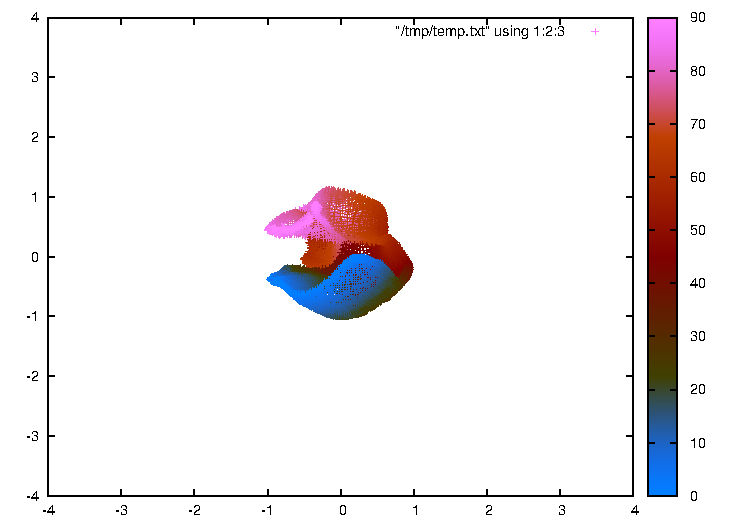
\includegraphics[scale=0.5,trim = 120 100 130 70, clip]{./figures/slow/drlim1.pdf}
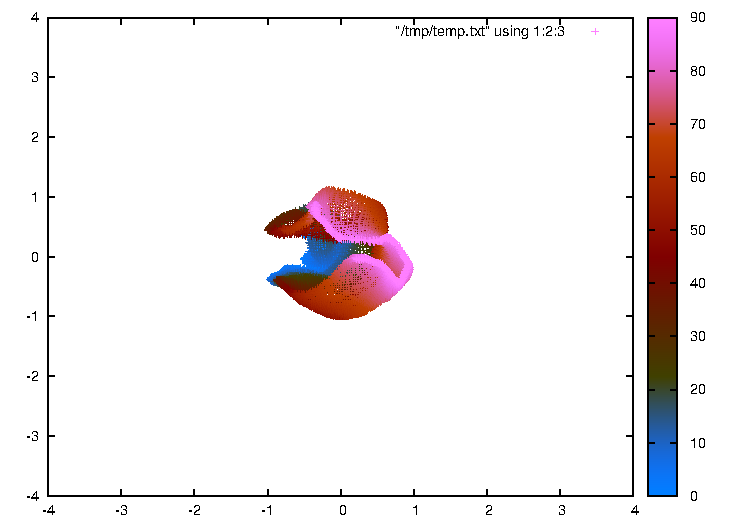
\includegraphics[scale=0.5,trim = 120 100 130 70, clip]{./figures/slow/drlim2.pdf}\\
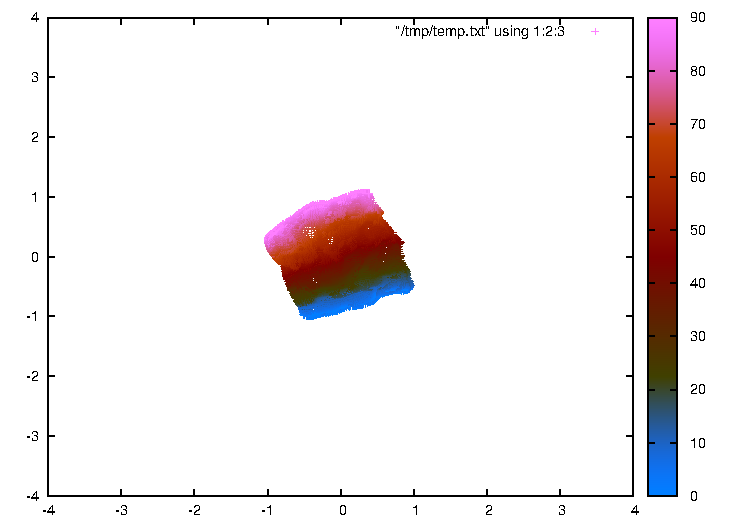
\includegraphics[scale=0.5,trim = 120 100 130 70, clip]{./figures/slow/drlim3.pdf} 
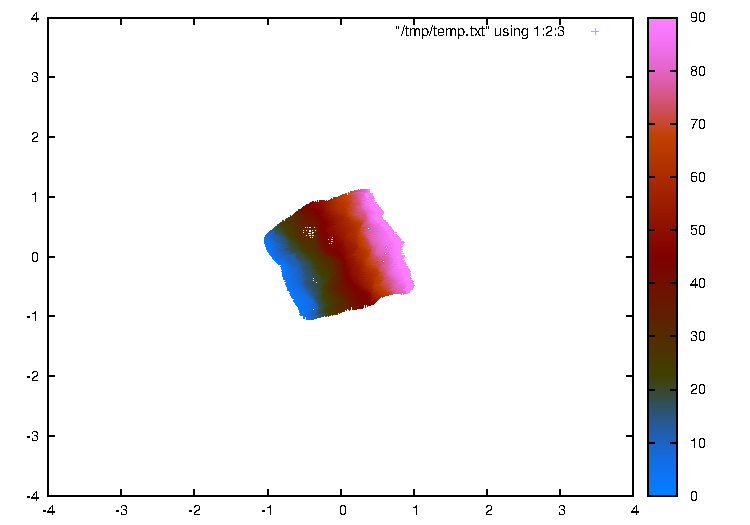
\includegraphics[scale=0.5,trim = 120 100 130 70, clip]{./figures/slow/drlim4.pdf}
        \caption{}
        \label{fig:drlim} 
\end{subfigure}

\caption{(a) Three samples from our rotating plane toy dataset. (b) Scatter plot of the dataset plotted in the output space of $G_W$ at the start (top) and end (bottom) of training. The left side of the figure is colored by the yaw angle, and the right side by roll, $0^{\circ}$  blue, $90^{\circ}$ in pink.}  
\end{figure} 

% Maybe reword so its not repetitive (first sent.) Temporal
coherence can be exploited by assuming a prior on the features extracted from
the temporal data sequence. One such prior is that the features should vary
slowly with respect to time. In the discrete time setting this prior
corresponds to minimizing an $L^p$ norm of the difference of feature vectors
for temporally adjacent inputs.  Consider a video sequence with $T$ frames, if
$z_t$ represents the feature vector extracted from the frame at time $t$ then
the slowness prior corresponds to minimizing $\sum_{t=1}^{T} \| z_t - z_{t-1}
\|_p$. To avoid the degenerate solution $z_t = z_0 ~\mbox{for}~ t=1...T$, a
second term is introduced which encourages data samples that are \emph{not}
temporal neighbors to be separated by at least a distance of $m$-units in
feature space, where $m$ is known as the margin. In the temporal setting this
corresponds to minimizing $max(0,m-\|z_t - z_{t'}\|_p)$, where $|t-t'| > 1$.
Together the two terms form the loss function introduced in \cite{DrLIM} as a
dimension reduction and data visualization algorithm known as DrLIM.  Assume
that there is a differentiable mapping from input space to feature space which
operates on \emph{individual} temporal samples. Denote this mapping by $G$ and
assume it is parametrized by a set of trainable coefficients denoted by $W$.
That is, $z_t = G_W(x_t)$. The per-sample loss function can be written as:
\begin{equation} \label{eqn:drlimcrit} L(x_t,x_{t'},W)=\left\{
\begin{array}{ll} \|G_W(x_t) - G_W(x_{t'})\|_p, &\text{if}~|t-t'| = 1  \\
\max(0,m-\|G_W(x_t) - G_W(x_{t'})\|_p) &\text{if}~|t-t'| > 1 \end{array}
\right.  \end{equation} In practice the above loss is minimized by constructing
a "Siamese" network (\cite{siamese}) with shared weights whose inputs are pairs
of samples along with their temporal indices. The loss is minimized with
respect to the trainable parameters with stochastic gradient descent via
back-propagation. To demonstrate the effect of minimizing Equation
\ref{eqn:drlimcrit} on temporally coherent data, consider a toy data-set
consisting of only one object. The data-set is generated by rotating a 3D model
of a toy plane (Figure \ref{fig:toyplane}) by $90^{\circ}$ in one-degree
increments around two-axes of rotation, generating a total of 8100 data
samples. Input images ($96 \times 96$) are projected into two-dimensional
output space by the mapping $G_W$. In this example the mapping $G_W(X):
\mathbb{R}^{9216} \to \mathbb{R}^2 $. We chose $G_W$ to be a fully connected
two layer neural network. In effect this data-set lies on an intrinsically
two-dimensional manifold parametrized by two rotation angles. Since the
sequence was generated by continuously rotating the object, temporal neighbors
correspond to images of the object in similar configurations.  Figure
\ref{fig:drlim} shows the data-set plotted in the output space of $G_W$ at the
start (top row) and end (bottom row) of training. The left and right hand sides
of Figure~\ref{fig:drlim} are colorized by the two rotational angles, which are
never explicitly presented to the network. This result implies that $G_W$ has
learned a mapping in which the latent variables (rotation angles) are
linearized. Furthermore, the gradients corresponding to the two rotation angles
are nearly orthogonal in the output space, which implies that the two features
extracted by $G_W$ are independent.  

\section{Slow Feature Pooling Auto-Encoders} \label{sfautoencs} The second
contrastive term in Equation \ref{eqn:drlimcrit} only acts to avoid the
degenerate solution in which $G_W$ is a constant mapping, it does not guarantee
that the resulting feature space is informative with respect to the input.
This discriminative criteria only depends on pairwise distances in the
representation space which is a geometrically weak notion in high dimensions.
We propose to replace this contrastive term with a term that penalizes the
reconstruction error of both data samples.  Introducing a reconstruction terms
not only prevents the constant solution but also acts to explicitly preserve
information about the input.  This is a useful property of features which are
obtained using unsupervised learning; since the task to which these features
will be applied is not known a priori, we would like to preserve as much
information about the input as possible. 

What is the optimal architecture of $G_{W}$ for extracting slow features? Slow
features are invariant to temporal changes by definition. In natural video and
on small spatial scales these changes mainly correspond to local translations
and deformations. Invariances to such changes can be achieved using appropriate
pooling operators \cite{JoanScat,LeCun1998}.  Such operators are at the heart
of deep convolutional networks (ConvNets), currently the most successful
supervised feature learning architectures \cite{ImageNet}. Inspired by these
observations, let $G_{W_e}$ be a two stage encoder comprised of a learned,
generally over-complete, linear map ($W_e$) and rectifying nonlinearity
$f(\cdot)$, followed by a local pooling. Let the $N$ hidden activations, $h =
f(W_ex)$, be subdivided into $K$ potentially overlapping neighborhoods denoted
by $P_i$. Note that biases are absorbed by expressing the input $x$ in
homogeneous coordinates. Feature $z_i$ produced by the encoder for the input at
time $t$ can be expressed as $G_{W_e}^i(t) = \|h_t\|^{P_i}_p =\left(\sum_{j \in
P_i} h_{tj}^{p} \right)^{\frac{1}{p}}$. Training through a local pooling
operator enforces a local topology on the hidden activations, inducing units
that are pooled together to learn complimentary features. In the following
experiments we will use $p=2$. Although it has recently been shown that it is
possible to recover the input when $W_e$ is sufficiently redundant,
reconstructing from these coefficients corresponds to solving a phase recovery
problem \cite{JoanPooling} which is not possible with a simple inverse mapping,
such as a linear map $W_d$. Instead of reconstructing from $z$ we reconstruct
from the hidden representation $h$. This is the same approach taken when
training group-sparse auto-encoders \cite{groupSparsity}. In order to promote
sparse activations in the case of over-complete bases we additionally add a
sparsifying $L_1$ penalty on the hidden activations. Including the rectifying
nonlinearity becomes critical for learning sparse inference in a hugely
redundant dictionary, e.g. convolutional dictionaries \cite{LISTA}. The
complete loss functional is: \begin{equation} \label{eqn:loss} L(x_t,x_{t'},W)=
\sum_{\tau = \{t,t'\}} \left(\|W_d h_\tau - x_\tau\|^2 + \alpha|h_\tau|
\right)+\beta \sum_{i=1}^K \left| \|h_t \|^{P_i} - \|h_{t'}\|^{P_i} \right|
\end{equation} Figure \ref{fig:diagram} shows a convolutional version of the
proposed architecture and loss.  This combination of loss and architecture can
be interpreted as follows: the sparsity penalty induces the first stage of the
encoder, $h=f(W_ex)$, to approximately infer sparse codes in the analysis
dictionary $W_e$; the slowness penalty induces the formation of pool groups
whose output is stable with respect to temporal deformations. In other words,
the first stage partitions the input space into disjoint linear subspaces and
the second stage recombines these partitions into temporally stable groups.
This can be seen as a sparse auto-encoder whose pooled codes are additionally
regularized by slowness.

\begin{figure} \centering \begin{subfigure}[b]{0.45\textwidth}
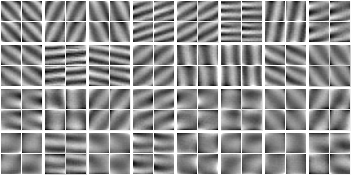
\includegraphics[width=\textwidth]{./figures/slow/slow_dec_pooling_sub.png}
\caption{} \label{fig:pooldec} \end{subfigure}
\begin{subfigure}[b]{0.45\textwidth}
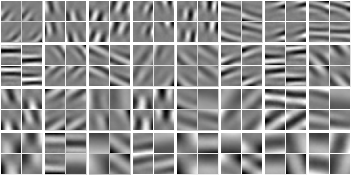
\includegraphics[width=\textwidth]{./figures/slow/slow_dec_l1_pooling.png}
\caption{} \label{fig:pooll1dec} \end{subfigure} \caption{Pooled decoder
dictionaries learned without (a) and with (b) the $L_1$ penalty using
(\ref{eqn:loss}).} \label{fig:sfpool} \end{figure}

\subsection{Fully-Connected Architecture}

To gain an intuition for the properties of the minima of Equation
\ref{eqn:loss} for natural data, an auto-encoder was trained on a small dataset
consisting of natural movie patches. This data set consists of approximately
170,000, $20 \times 20$ gray scale patches extracted from full resolution
movies.  Minimizing Equation \ref{eqn:loss} with $\alpha=0$ results in the
learned decoder basis shown in Figure \ref{fig:pooldec}. Here a dictionary of
512 basis elements was trained whose outputs were pooled in non-overlapping
groups of four resulting in 128 output features. Only the slowest 32 groups are
shown in Figure \ref{fig:pooldec}. The learned dictionary has a strong
resemblance to the two-dimensional Fourier basis, where most groups are
comprised of phase shifted versions of the same spatial frequency. Since
translations are an invariant of the local modulus of the Fourier transform,
the result of this experiment is indicative of the fact that translations are
the principal source of variation at small spatial scales. Minimizing Equation
\ref{eqn:loss} with $\alpha > 0$ results in a more localized basis depicted in
Figure \ref{fig:pooll1dec}. This basis is more consistent with a local
deformation model as opposed to a global one. 

\subsection{Convolutional Architecture} By replacing all linear operators in
our model with convolutional filter banks and including spatial pooling,
translation invariance need not be learned \cite{LeCun1998}. In all other
respects the convolutional model is conceptually identical to the fully
connected model described in the previous section. One important difference
between fully-connected and convolutional dictionaries is that the later can be
massively over-complete, making sparse inference potentially more challenging.
Nevertheless we found that non-trivial dictionaries (see Figure
\ref{fig:slowfilters}) can be learned using purely stochastic optimization,
that is, without a separate sparse inference phase. Let the linear stage of the
encoder consist of a filter bank which takes $C$ input feature maps
(corresponding to the 3 color channels for the first stage) and produces $D$
output feature maps. Correspondingly, the convolutional decoder transforms
these $D$ feature maps back to $C$ color channels. In the convolutional setting
slowness is measured by subtracting corresponding spatial locations in
temporally adjacent feature maps. In order to produce slow features a
convolutional network must compensate for the motion in the video sequence by
producing \emph{spatially} aligned activations for \emph{temporally} adjacent
samples. In other words, in order to produce slow features the network must
implicitly learn to track common patterns by learning features which are
invariant to the deformations exhibited by these patterns in the temporal
sequence. The primary mechanism for producing these invariances is pooling in
space and across features \cite{MaxOut}. Spatial pooling induces local
translation invariance. Pooling across feature maps allows the network to
potentially learn feature groups that are stable with respect to more general
deformations. Intuitively, maximizing slowness in a convolutional architecture
leads to \emph{spatiotemporally} coherent features.  
\begin{figure} \centering
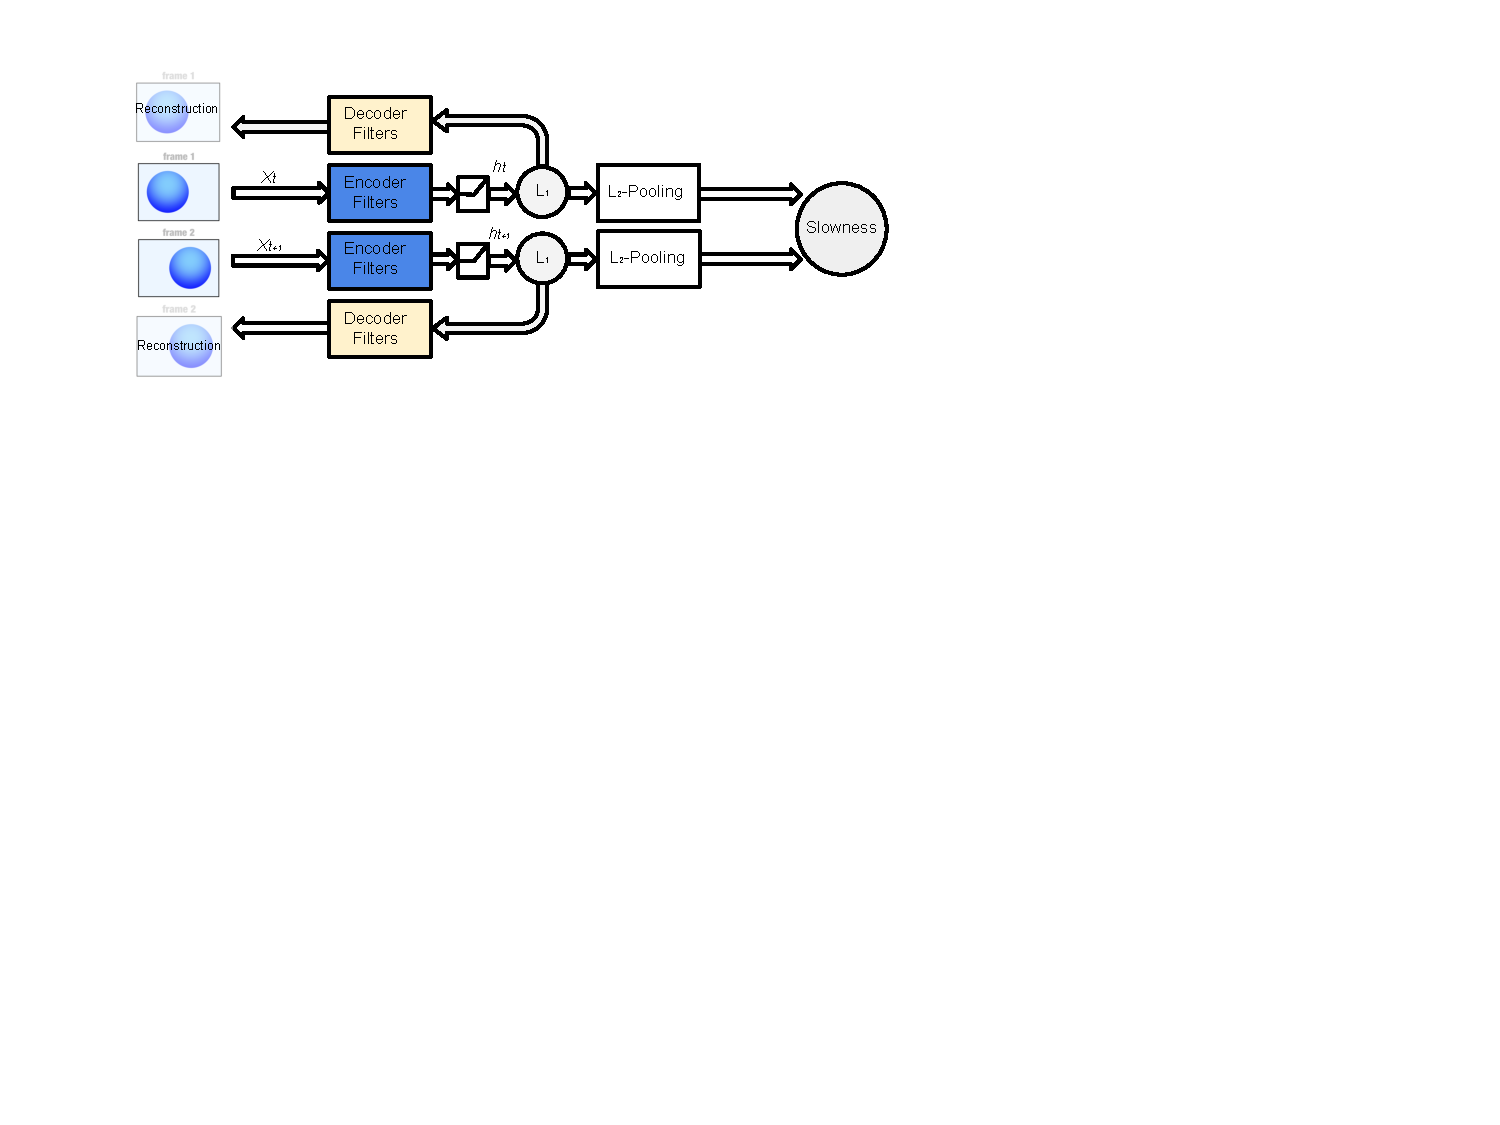
\includegraphics[scale=0.75,trim = 15 350 290 39,clip]{./figures/slow/Rebbutal_Figures/diagram.pdf} \caption{Block diagram of the Siamese convolutional model trained on pairs of frames. 
\label{fig:diagram}}
\end{figure} 
\section{Experimental Results} To verify the connection between
slowness and metric learning, we evaluate the metric properties of the learned
features. It is well known that distance in the extrinsic (input pixel) space
is not a reliable measure of semantic similarity. Maximizing slowness
corresponds to minimizing the distance between adjacent frames in code space,
therefore neighbors in code space should correspond to temporal neighbors. This
claim can be tested by computing the nearest neighbors to a query frame in code
space, and verifying whether they correspond to its temporal neighbors.
However, the features must also be discriminative so as not to collapse
temporally distant samples. In order to make this trade-off in a principled
manner, a dataset comprised of short natural scenes was collected.
Hyper-parameters are selected which maximize the so called "temporal coherence"
of the features which define the metric. We define the temporal coherence of a
metric $G_W(\cdot)$ as the area under the precision-recall curve, where
precision is defined as the proportion of the nearest neighbors that come from
the same scene, and recall is defined as the proportion of frames recalled from
that scene. In our experiments, we used the middle frame from each scene as the
query. 

However, temporal coherence can be a very weak measure of discriminability; it
merely requires that scenes be easy to disambiguate in feature space. If the
scenes are quite distinct, then maximizing temporal coherence directly can lead
to weakly discriminative features (e.g.~color histograms can exhibit good
temporal coherence). We therefore evaluate the learned features on a more
demanding task by assessing how well the metric learned from the YouTube
dataset transfers to a classification task on the CIFAR-10 dataset. Average
class-based precision is measured in feature space by using the test set as the
query images and finding nearest neighbors in the training set. Precision is
defined as the proportion of nearest neighbors that have the same label. As on
the YouTube dataset we evaluate the average precision for the nearest 40
neighbors. The CIFAR dataset contains considerably more interclass variability
than the scenes in our YouTube dataset, nevertheless many class instances are
visually similar.  

%\subsection{Description of Experiments} Our training dataset consists of
approximately $150,000$ frames extracted from YouTube videos. Of these,
approximately $20,000$ frames were held out for testing. The training and test
set frames were collected from separate videos. The videos were automatically
segmented into scenes of variable length (2-40 frames) by detecting large $L_2$
changes between adjacent frames. Each color frame was down-sampled to a $32
\times 32$ spatial resolution and the entire dataset was ZCA whitened
\cite{alexthesis}. Six scenes from the test set are shown in Figure
\ref{fig:youtube} where the first scene (top row) is incorrectly segmented.   

We compare the features learned by minimizing the loss in Equation
\ref{eqn:loss} with the features learned by minimizing DrLIM (Equation
\ref{eqn:drlimcrit}) and group sparsity (Equation \ref{eqn:groupL1}) losses.
Once trained, the convolution, rectification, and pooling stages are used to
transform the dataset into the feature space. We use cosine distance in feature
space to determine the nearest neighbors and select hyperparmeters for each
method which maximize the temporal coherence measure.

We trained two layers of our model using greedy layer-wise training
\cite{Bengio2012}. The first layer model contains a filter bank consisting of
64 kernels with $9 \times 9$ spatial support. The first $L_2$ pooling layer
computes the local modulus volumetrically, that is \emph{across} feature maps
in non-overlapping groups of four and spatially in $2 \times 2$ non-overlapping
neighborhoods. Thus the output feature vector of the first stage ($z_1$) has
dimensions $16 \times 16 \times 16$ (4096). Our second stage consists of 64 $5
\times 5$ convolutional filters, and performs $4 \times 4$ spatial pooling
producing a second layer code ($z_2$) of dimension $64 \times 4 \times 4$
(1024). The output of the second stage corresponds to a dimension reduction by
a factor of three relative to the input dimension.

Identical one and two-layer architectures were trained using the group sparsity
prior, similar to \cite{groupSparsity}. As in the slowness model, the two layer
architecture was trained greedily. Using the same notation as Equation
\ref{eqn:loss}, the corresponding loss can be written as:  \begin{equation}
L(x_t,W)= \sum_{\tau} \|W_d h_\tau - x_\tau\|^2 +\alpha \|h_\tau \|^{P_i}
\label{eqn:groupL1} \end{equation} Finally, identical one and two-layer
architectures were also trained by minimizing the DrLIM loss in Equation
\ref{eqn:drlimcrit}. Negative pairs, corresponding to temporally non-adjacent
frames, were independently selected at random. In order to achieve the best
temporal precision-recall performance, we found that each mini-batch should
consist of a large proportion of negative to positive samples (at least
five-to-one). Unlike the auto-encoder methods, the two layer architecture was
trained jointly rather than greedily.  \begin{figure} \centering
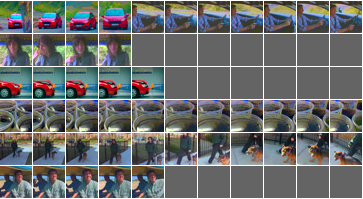
\includegraphics[scale=0.5]{./figures/slow/youtube.png} \caption{Six scenes from our
YouTube dataset \label{fig:youtube}}  \end{figure} \begin{figure}[ht]
\centering \newcommand{\figspace}{0.0cm} \newcommand{\figsize}{0.24\textwidth}
\begin{subfigure}[b]{\figsize}
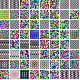
\includegraphics[width=\textwidth]{./figures/slow/Rebbutal_Figures/filters_drlim.png}
\caption{} \label{fig:drlimfilters} \end{subfigure} \hspace{\figspace}
\begin{subfigure}[b]{\figsize}
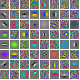
\includegraphics[width=\textwidth]{./figures/slow/filters_not_slow.png} \caption{}
\label{fig:L1filters} \end{subfigure} \hspace{\figspace}
\begin{subfigure}[b]{\figsize}
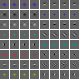
\includegraphics[width=\textwidth]{./figures/slow/Rebbutal_Figures/filters_group_sparse.png}
\caption{} \label{fig:groupL1filters} \end{subfigure} \hspace{\figspace}
\begin{subfigure}[b]{\figsize}
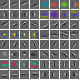
\includegraphics[width=\textwidth]{./figures/slow/filters_slow.png} \caption{}
\label{fig:slowfilters} \end{subfigure} \caption{Pooled convolutional
dictionaries (decoders) learned with: (a) DrLIM and (b) sparsity only, (c)
group sparsity, and (d) sparsity and slowness. Groups of four features that
were pooled together are depicted as horizontally adjacent filters.}
\label{fig:filters} \end{figure}

\begin{figure} \center \begin{subfigure}[b]{0.45\textwidth}
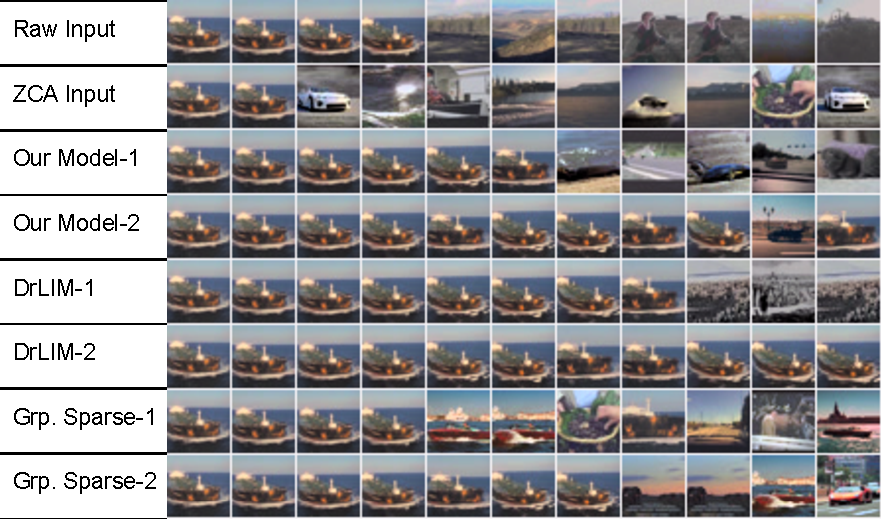
\includegraphics[width=\textwidth, trim = 0 0 34 0,
clip]{./figures/slow/Rebbutal_Figures/NNtime1.pdf} 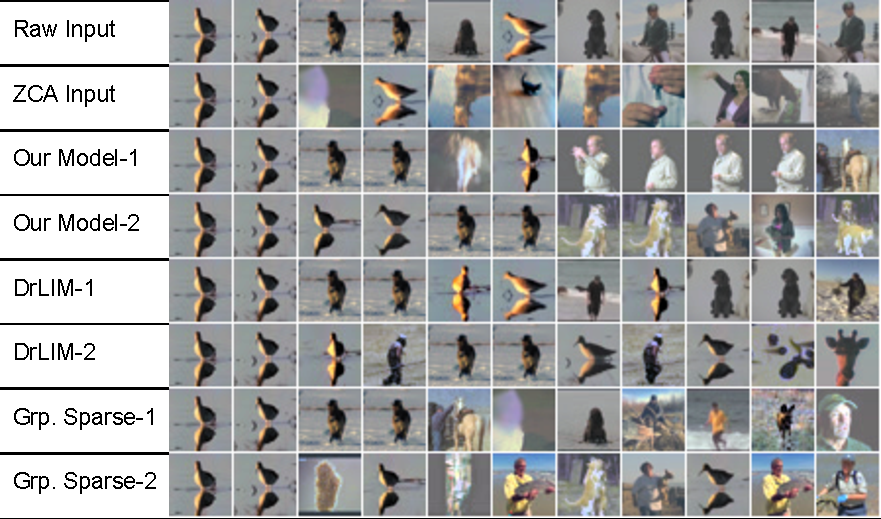
\includegraphics[width=\textwidth, trim =
0 0 34 0, clip]{./figures/slow/Rebbutal_Figures/NNtime2.pdf} \caption{}
\label{fig:videoquery} \end{subfigure} \centering \hspace{0.1cm}
\begin{subfigure}[b]{0.45\textwidth} 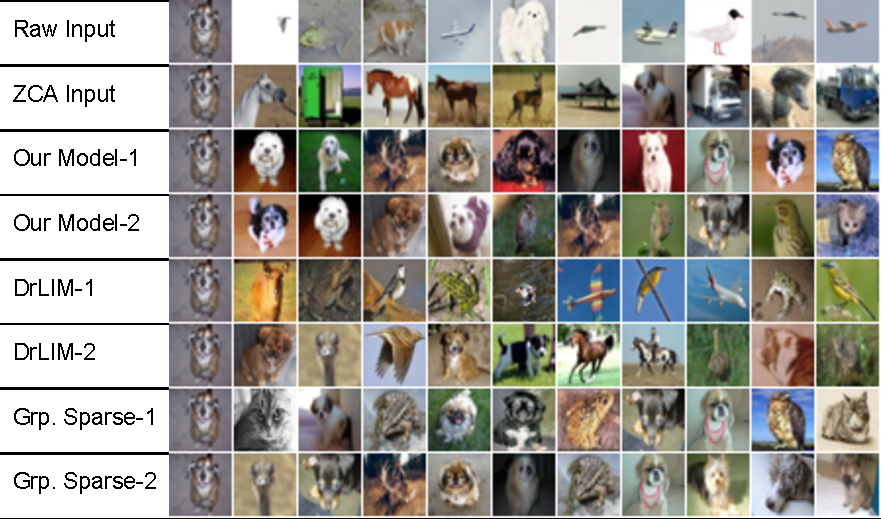
\includegraphics[width=\textwidth, trim =
0 0 34 0, clip]{./figures/slow/Rebbutal_Figures/NNclass1.pdf}
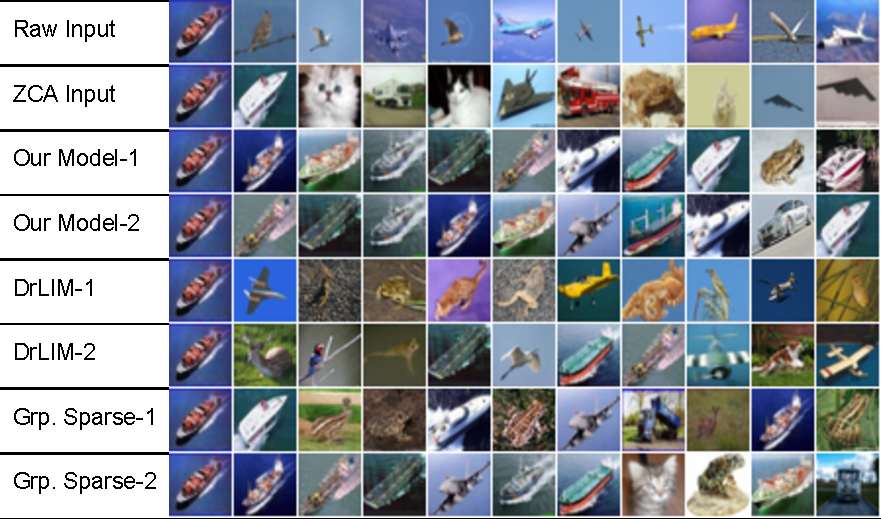
\includegraphics[width=\textwidth, trim = 0 0 34 0,
clip]{./figures/slow/Rebbutal_Figures/NNclass2.pdf} \caption{} \label{fig:cifarquery}
\end{subfigure} \caption{Query results in the (a) video and (b) CIFAR-10
datasets. Each row corresponds to a different feature space in which the
queries were performed; numbers (1 or 2) denote the number of
convolution-pooling layers. \label{fig:query}}  \label{fig:query} \end{figure}

\begin{figure} \centering \begin{subfigure}[b]{0.45\textwidth}
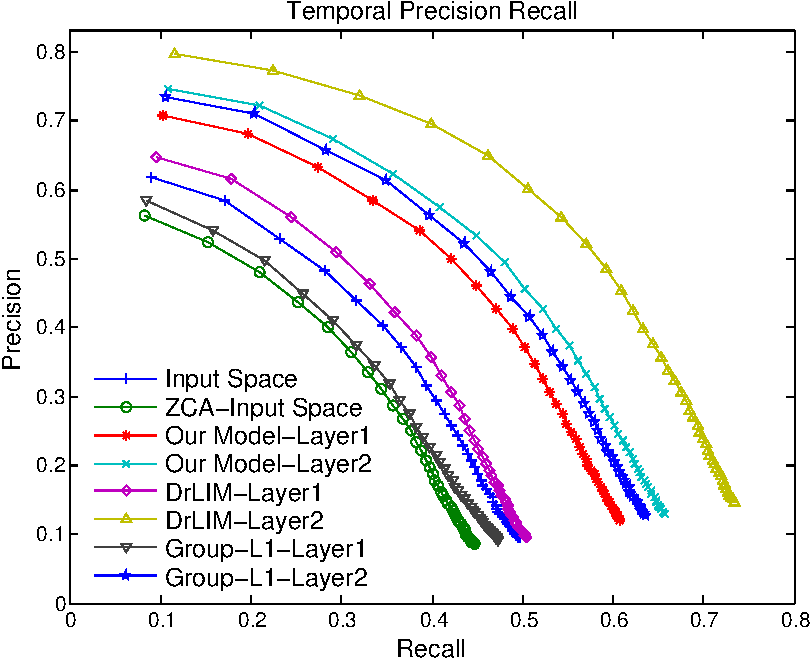
\includegraphics[width=\textwidth]{./figures/slow/Rebbutal_Figures/AUC_time-crop.pdf}
\caption{} \label{fig:ROCtime} \end{subfigure} \centering
\begin{subfigure}[b]{0.45\textwidth}
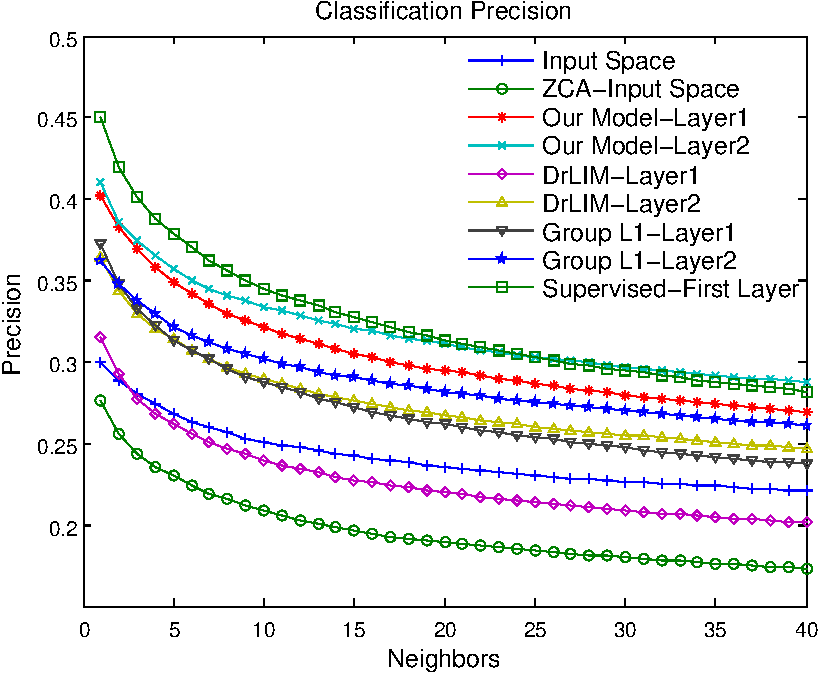
\includegraphics[width=\textwidth]{./figures/slow/Rebbutal_Figures/AUC_class-crop.pdf}
\caption{} \label{fig:ROCCIFAR} \end{subfigure} \caption{Precision-Recall
curves corresponding to the YouTube (a) and CIFAR-10 (b) dataset.}
\label{fig:ROC} \end{figure}

\begin{table} \centering \begin{tabular}{| l | l | l | l |} \hline Model &
Optimization & Temporal AUC & Class AUC \\ \hline Our Model Layer1 & --- &
0.262 & 0.296 \\ Our Model Layer2 & Greedy & 0.300 & \bf{0.310} \\ DrLIM Layer1
& --- & 0.188 & 0.221 \\ DrLIM Layer2 & Joint & \bf{0.378} & 0.268 \\ Group
$L_1$ Layer1 & --- & 0.231 & 0.266 \\ Group $L_1$ Layer2 & Greedy & 0.285 &
0.281 \\ \hline \end{tabular} \caption{Comnparison of Temporal and Class AUCs} \end{table} %\subsection{Discussion of Results}
%filter discussion  Figure \ref{fig:videoquery} shows the top nine query
results on the YouTube dataset for a single frame (left column) in eight
spaces. The top row shows the nearest neighbors in pixel space. The second row
shows the nearest neighbors in pixel space after ZCA whitening. The next six
rows show the nearest neighbors in feature space for one and two layer feature
transformations learned with slowness, group sparsity, and DrLIM. The resulting
first-layer filters and precision-recall curves are shown in Figures
\ref{fig:filters} and \ref{fig:ROC}, respectively.   Figures
\ref{fig:L1filters} and \ref{fig:slowfilters} show the decoders of two
one-layer models trained with $\beta = 0,2$, respectively, and a constant value
of $\alpha$. The filter bank trained with $\beta = 0$ exhibits no coherence
within each pool group; the filters are not visually similar nor do they tend
to co-activate at spatially neighboring locations. Most groups in the filter
bank trained with slowness tend be visually similar, corresponding to similar
colors and/or geometric structures. The features learned by minimizing the
DrLIM loss (Equation \ref{eqn:drlimcrit}), which more directly optimizes
temporal coherence, have much more high frequency content than the filters
learned with any of the auto-encoder methods. Nevertheless, some filters within
the same pool group exhibit similar geometric and color structure
(Figure~\ref{fig:drlimfilters}). The features learned with a group-sparsity
regularizer leads to nearly identical features (and nearly identical
activations) within each pool group (Figure~\ref{fig:groupL1filters}). This is
not surprising because group sparsity promotes co-activation of the features
within each pool group, by definition. We have also tried including an
individual sparsity prior, as in Equation~\ref{eqn:loss}, in order to encourage
independence among the pooled features. However this has lead to significantly
worse temporal-coherence performance.  %AUC discussion 

Figure \ref{fig:cifarquery} shows the result of two queries in the CIFAR-10
dataset. The corresponding precision-recall curves are shown in Figure
\ref{fig:ROCCIFAR}. One-layer DrLIM (4096 dimensional) exhibit poor performance
in both the temporal and class-based recall tasks. In contrast, jointly trained
two-layer DrLIM features (1024 dimensional) exhibit excellent temporal
coherence, outperforming all other models by a large margin. Although better
than the  first layer, second layer features perform significantly worse on the
CIFAR task than even the first-layer features learned by our model.
Furthermore, the nearest neighbors in both the one and two-layer feature spaces
learned with DrLIM are often neither visually nor semantically similar (see
Figure \ref{fig:cifarquery}). The conclusion which can be drawn from this
result is that \textbf{\emph{directly maximizing temporal coherence alone is
not a sufficient condition for achieving a semantically (or even visually)
coherent features}}. However, combining it with reconstruction and sparsity, as
in our model, yields the most semantically discriminative features. Although
significantly better than the features learned with DrLIM, the features learned
with group sparsity exhibit slightly weaker temporal coherence and
significantly worse class-based recall. Note that since all the features within
a pool group are practically identical, the invariants captured by the pool
groups are limited to local translations due to the spatial pooling. As a final
comparison, we trained a four layer ConvNet with supervision on CIFAR-10, this
network achieved approximately 80\% classification accuracy on the test set.
The architecture of the first two stages of the ConvNet is identical to the
architecture of the first and second unsupervised stages. The precision curve
corresponding to the first layer of the ConvNet is shown in Figure
\ref{fig:ROCCIFAR}, which is matched by our-model's second layer at high
recall. 

\section{Conclusion} Video data provides a virtually infinite source of
information to learn meaningful and complex visual invariances. While temporal
slowness is an attractive prior for good visual features, in practice it
involves optimizing conflicting objectives that balance invariance and
discriminability. In other words, perfectly slow features cannot be
informative. An alternative is to replace the small temporal velocity prior
with small temporal acceleration, leading to a criteria that \emph{linearizes}
observed variability. The resulting representation offers potential advantages,
such as extraction of both locally invariant and locally covariant features.
Although pooling representations are widespread in visual and audio recognition
architectures, much is left to be understood. In particular, a major question
is how to learn a stacked pooling representation, such that its invariance
properties are boosted while controlling the amount of information lost at each
layer. This could be possible by replacing the linear decoder of the proposed
model with a non-linear decoder which can be used to reconstruct the input from
pooled representations. Slow feature learning is merely one way to learn from
temporally coherent data. In this work we have provided an auto-encoder
formulation of the problem and shown that the resulting features are more
stable to naturally occurring temporal variability, while maintaining
discriminative power.
